% Created 2019-02-15 Fri 12:13
% Intended LaTeX compiler: pdflatex
\documentclass[11pt]{article}
\usepackage[utf8]{inputenc}
\usepackage[T1]{fontenc}
\usepackage{graphicx}
\usepackage{grffile}
\usepackage{longtable}
\usepackage{wrapfig}
\usepackage{rotating}
\usepackage[normalem]{ulem}
\usepackage{amsmath}
\usepackage{textcomp}
\usepackage{amssymb}
\usepackage{capt-of}
\usepackage{hyperref}
\usepackage{geometry}
\geometry{a4paper, textwidth=6.5in, textheight=10in, marginparsep=7pt, marginparwidth=.6in}
\setlength{\parskip}{12pt}
\hypersetup{colorlinks=true}
\author{Rakhim Davletkaliyev}
\date{\today}
\title{Notes on Bartosz Milewski - Truth about Types (Lambda Days 2016)}
\hypersetup{
 pdfauthor={Rakhim Davletkaliyev},
 pdftitle={Notes on Bartosz Milewski - Truth about Types (Lambda Days 2016)},
 pdfkeywords={},
 pdfsubject={},
 pdfcreator={Emacs 26.1 (Org mode 9.1.9)},
 pdflang={English}}
\begin{document}

\maketitle
\tableofcontents


\section{Intro}
\label{sec:org6d8c16f}

Category theory abstracts many branches of math. You can describe topology, logic, Banach spaces and other concepts in terms of category theory. Why is it so? Does category theory describe the nature, the intrinsic reality, and we happened to discover it like physicists discover the laws of the universe?

The main idea of category theory is composition. This is why it is so relevant in programming. Composition is the essence of category theory.

Is composability intrinsic in nature? It seems like that on a larger scale, and classical physics shows how everything is neatly composable. The ancient idea of atoms is the idea of perfect composability: things are composed with indivisible elementary particles, and the higher you go, the more composable everything is. Atoms make molecules, molecules make objects, object make bigger objects and interact using laws that are themselves composable. Newtonian mechanics describes objects in the universe that follow the rules of interaction that are clearly affecting each other, acting like independent agents.

But the deeper you go, the less composable it becomes. Two quantum particles don't interact in a simply composable fashion, their wave functions do not just affect each other in a stable manner. Two quantum particles near one another start to behave like a special two-particle state, not two wave functions. This is why quantum theory is so hard to describe and this is probably why physicists struggle with these theories. They go against our intuition of a composable universe.

So, maybe composability is not intrinsic in nature, maybe it is intrinsic for our limited monkey brains. We need composability in order to deal with the complex reality. Maybe, higher super-beings wouldn't invent category theory at all.

\section{Truth}
\label{sec:org0633929}

In logic, there is an axiom that basically says "truth is true", and you don't need to prove it.

\begin{eqnarray}
\frac{}{\top true}\top_I
\end{eqnarray}

In type theory, it corresponds to unit type:

\begin{eqnarray}
():()
\end{eqnarray}

And in category theory it corresponds to the terminal object, which we will cover later.

Three things look different, but they are actually just different notations for the same concept.

As for proofs, in logic you'd prove a proposition A by providing some statements:

\begin{eqnarray}
\frac{[...]}{A}
\end{eqnarray}

In type theory, you'd prove that type \textbf{A} is inhabited (has members):

\begin{eqnarray}
\Gamma\vdash x : A
\end{eqnarray}

In the context of categories, a proof would be a morphism from terminal object:

\begin{eqnarray}
1\rightarrow A
\end{eqnarray}

\section{Category theory}
\label{sec:orga02556f}

A \href{https://en.wikipedia.org/wiki/Category\_theory}{category} is a collection of objects and arrows.

Similar to a directed \href{https://en.wikipedia.org/wiki/Graph\_theory}{graph}. Nodes are called \textbf{objects} (a, b, c,\ldots{}). Arrows between objects are called \textbf{morphisms}: \texttt{f :: a -> b}.

\subsection{Composability}
\label{sec:orgc594467}

Arrows are composable:

\begin{eqnarray}
f :: a \rightarrow b
\end{eqnarray}
\begin{eqnarray}
g :: b \rightarrow c
\end{eqnarray}
\begin{eqnarray}
g \circ f :: a \rightarrow c
\end{eqnarray}

The notation \(g \circ f\) means "apply \texttt{g} after \texttt{f}".

So, composition is associative.

\subsection{Identity arrows}
\label{sec:orge61eaac}

There always exist identity arrows that point to the same object:

\begin{eqnarray}
id_a :: a \rightarrow a
\end{eqnarray}

\begin{eqnarray}
id \circ f = f
\end{eqnarray}

\begin{eqnarray}
g \circ id = g
\end{eqnarray}

There could be multiple arrows from \texttt{a} to \texttt{a}, but at least one is identity.

\subsection{Set}
\label{sec:org8b284b5}

\href{https://en.wikipedia.org/wiki/Set\_theory}{Set} is an example of a category. Set is a category in which:
\begin{itemize}
\item Objects are sets
\item Arrows are functions
\end{itemize}

In category theory, you cannot "look" inside objects, you only care about their connections. So, two sets are considered to be the same or different based on the arrows, but not the contents.

\section{Universal constructions in category theory}
\label{sec:orgfb8900b}
\subsection{Initial object}
\label{sec:org802c37e}

An \href{https://en.wikipedia.org/wiki/Initial\_and\_terminal\_objects}{initial object} is an object that has a unique arrow to all other objects. Only one arrow per object.

\begin{center}
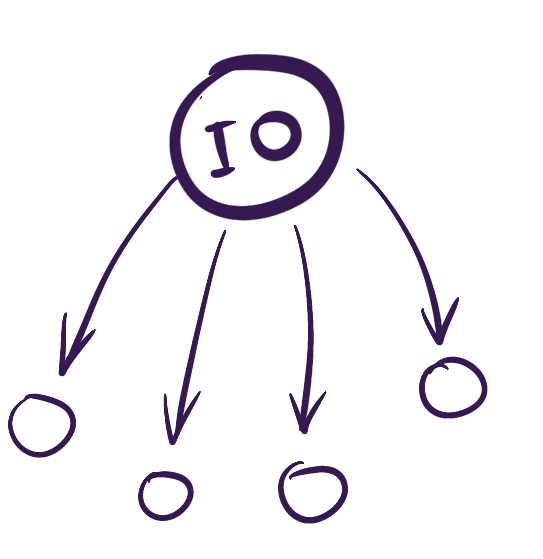
\includegraphics[width=2.0in]{./img/initial_object.png}
\end{center}

In Set, the equivalent would be an empty set \(\varnothing\). A function \(varnothing \rightarrow a\) is a function that maps an element of empty set to any other element of other set. This doesn't make sense: an element of empty set? But this is just an explanation in terms of set theory, and while it doesn't make sense, we can think about this nevertheless, as of "objects defined by their arrow property".

You can always create a function from an empty set, but you'll never be able to call this function. In the abstract, in vacuum this is true.

In Haskell there's Absurd function:

\begin{verbatim}
Absurd :: Void -> a
\end{verbatim}

Which is a reference to "ad absurdum": from falsehood, you can derive anythings. "If pigs can fly, then I am the president".

\texttt{Void} here represents a type \texttt{Void}, an uninhabited type. This is not the same void-type we use in C/C++.

\subsection{Terminal object}
\label{sec:org3c08bf8}

The inverse of initial object is the \href{https://en.wikipedia.org/wiki/Initial\_and\_terminal\_objects}{terminal object}. An object with a unique arrow from all objects.

\begin{center}
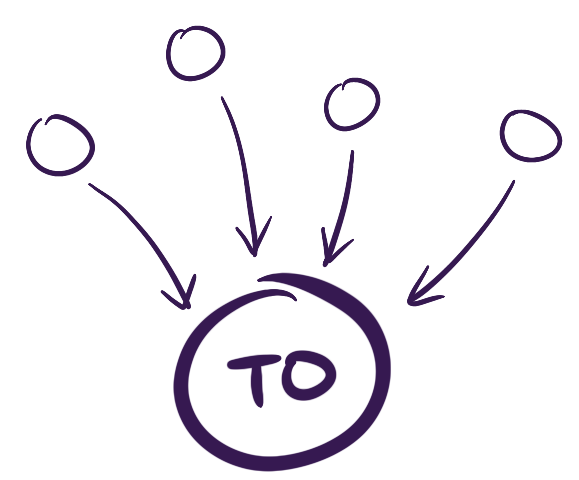
\includegraphics[width=2.0in]{./img/terminal_object.png}
\end{center}

In set, it's a singleton set. Unique function: for every element of set \textbf{a} return the single element of the singleton set. In Haskell, the unit function ignores the argument and returns the one element from the set. The unit type \texttt{()} has one element \texttt{()}.

Type:

\begin{verbatim}
unit :: a -> ()
\end{verbatim}

Element of this type:

\begin{verbatim}
unit _ -> ()
\end{verbatim}

If there are many singleton sets, they are isomorphic (i.e., a set of one apple is the same as a set of one orange).

\section{Product}
\label{sec:orgb10d3b5}

We need these universal constructions because they provide a way of defining things (since you cannot look inside the objects). One of the things that can be defined is the product.

\begin{itemize}
\item \texttt{c} is a product of \texttt{a} and \texttt{b}
\item two arrows \texttt{p} and \texttt{q} (projections)
\item in Set: Cartesian product, pairs of elements
\item in logic: logical \texttt{AND} (conjuction elimination)
\end{itemize}

\begin{center}
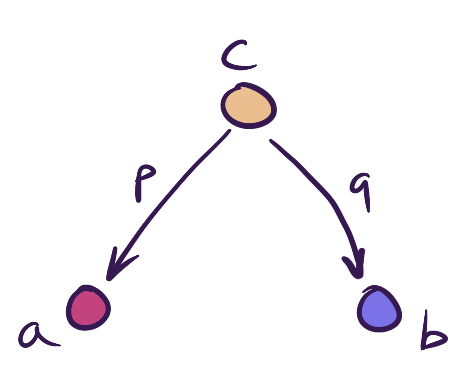
\includegraphics[width=2.0in]{./img/product.png}
\end{center}

The only thing we know is that there are two morphisms. If we translate this into logic, it corresponds exactly to the elimination (AND). If \texttt{a AND b} is true, then \texttt{a} is true:

\begin{eqnarray}
\frac{a \wedge b}{a}
\end{eqnarray}

If \texttt{a AND b} is true, \texttt{b} is true:

\begin{eqnarray}
\frac{a \wedge b}{b}
\end{eqnarray}

This corresponds to morphisms like so:

\begin{verbatim}
c :: (a, b)
p(a, b) = a
q(a, b) = b
\end{verbatim}

There can be many objects like \texttt{c} with such two projections. Only one could the product. Which one? We need to pinpoint the correct \texttt{c} that corresponds to the Cartesian product. We need a way to evaluate the instance of this pattern of projections.

If we can get all similar patterns in the category, we need a way to distinguish the "top" one, the one that matches the the best. That one would be the product.

Here we have two examples of such pattern:

\begin{center}
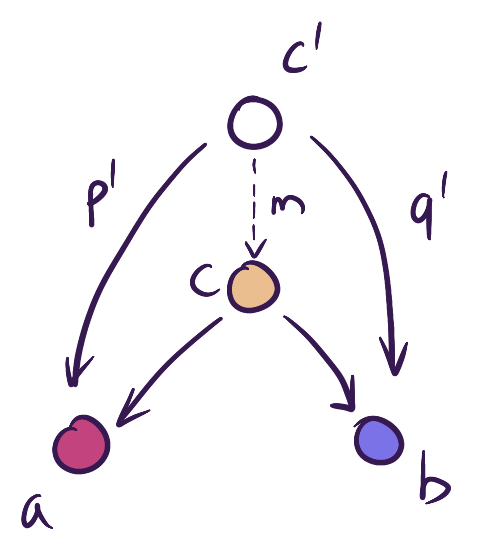
\includegraphics[width=2.0in]{./img/candidate.png}
\end{center}

\texttt{c'} is a candidate product and it has \texttt{p'} and \texttt{q'} projections. \texttt{c} is better if there is a unique arrow (morphism) \texttt{m} from \texttt{c'} to \texttt{c} that fulfils these conditions:

\begin{equation}
\begin{aligned}
m :: c' \rightarrow c \\
p' = p \circ m \\
q' = q \circ m
\end{aligned}
\end{equation}


Both of these have the common factor \texttt{m} (but instead of multiplication you have composition). So they are not really elementary, since we can factor out a common \texttt{m} out of them. This makes \texttt{c} better ("more pure").

This forms ranking among candidates. In some cases you can indeed use ranking to get the unique best option and that will be the product. Not all categories would have this.

Again, there is a connection to logic:

\begin{verbatim}
if a follows from c'       (p')
and b follows from c'      (q')
a ^ b (c) follows from c'  (m)
\end{verbatim}

\section{Function object}
\label{sec:org3e6631f}

Another universal construction.

What is type function in Haskell? It's not really a morphism. Morphism is not an object. A set of morphisms between two objects corresponds to type \texttt{a->b}. Is there an object in the category that corresponds to the set of morphisms? If so, it's called the Function Object.

In order to define the function object (in Haskell, it's \texttt{a->b}, which is a type), you have to have products.

\begin{center}
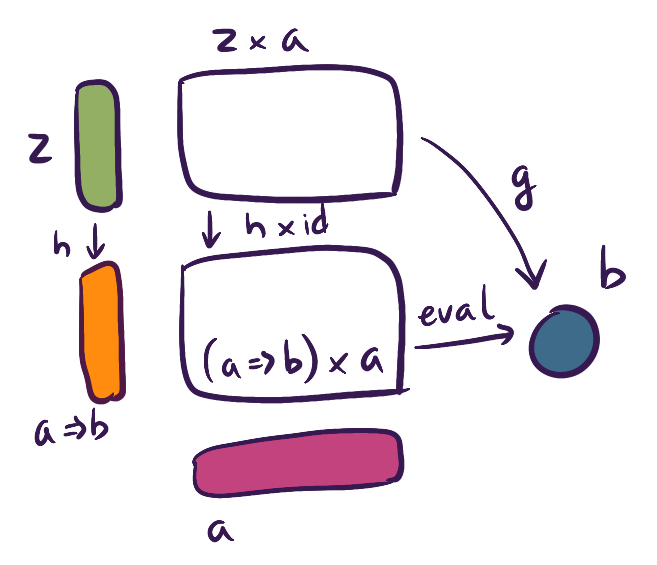
\includegraphics[width=3.0in]{./img/function.png}
\end{center}

If you take a function \texttt{a->b} and apply argument \texttt{a}, you get \texttt{b}. Similar to product, if there is another candidate object \texttt{z}, that evaluates to the same \texttt{b}, and you can find unique morphism \texttt{h} then you can factor it out and prove that \texttt{a->b} candidate is the best.

This corresponds to modus ponens in proof theory.

\begin{eqnarray}
\frac{(a=>b) \wedge a}{b}
\end{eqnarray}

If you have a function from \texttt{a} to \texttt{b} \textbf{and} \texttt{a} is true, then \texttt{b} is also true.

\section{Negation}
\label{sec:org6a533b2}

Another thing you can construct is negation. \texttt{Not A} corresponds to an arrow (morphism) \texttt{A -> Void}. Why is this a negation?

In the context of type theory:

\begin{itemize}
\item If \texttt{A} is inhabited (has elements), then \texttt{A->Void} is not inhabited. Because otherwise you'd be able to create an element of \texttt{Void}, which suppose to have no elements.
\item If \texttt{A} is not inhabited (is Void), then \texttt{Void->Void} is \(id_{void}\).
\end{itemize}

\section{Cartesian Closed Category}
\label{sec:org953cc8b}

Combining these three things, we get a Cartesian Closed Category (CCC):
\begin{itemize}
\item Has all products (Cartesian)
\item Has all function objects (exponentials) (this makes it closed)
\item Has terminal object (nullary product)
\end{itemize}

\section{Curry-Howard-Lambek}
\label{sec:org5b2cb02}

This is an extension of Curry-Howard isomorphism. CCC is a model for simply typed lambda calculus. In addition to the fact that simply typed lambda calculus can be a model for logic.

\begin{itemize}
\item Objects are types
\item Morphisms are terms (in logic/programming)
\item Environment \(\Gamma\) is a prodict of judgements \texttt{a:A}
\item Empty environment is \texttt{() : ()}
\end{itemize}

\section{Logical universes}
\label{sec:org1ee0905}

There are two major kinds of logic: Classical and Intuitionistic.

\begin{center}
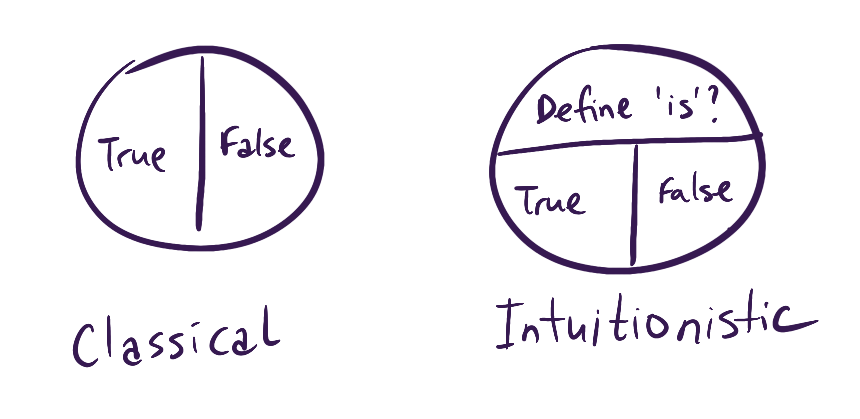
\includegraphics[width=3.0in]{./img/logics.png}
\end{center}

In classical logic, any proposition is either true or false. But then Kurt Gödel comes along and says "no, there are some statements that are neither false nor true", which leads to intuitionistic logic where a statement can be true, can be false, but you can also have some gray area where you ask what "is" means.

\subsection{Intuitionistic logic}
\label{sec:org70dafa2}
\begin{itemize}
\item No LEM: law of excluded middle (either A or not A). \texttt{A | (A->Void)} is not provable.
\item We cannot eliminate double negation: \texttt{Not Not A} is not the same as \texttt{A} (\texttt{(A->Void)->Void} is not the same as \texttt{A})
\end{itemize}

Curry-Howard equivalence says that simple typed lambda calculus is equivalent to intuitionistic logic. You cannot prove LEM or double negation using lambda calculus.

So, we cannot do classical logic? This means it's not relevant to programming then?

\subsection{Goedel Gentzen}
\label{sec:org45fe406}

Turns out, classical logic can be embedded in intuitionistic logic. Classical logic = Intuitionistic + double negation elimination (or LEM).

You can take a proposition in classical logic that is provable, you can translate it into some other proposition in intuitionistic logic, and then translate the proof also that does not use double negation elimination or LEM, and you will get something. There is a correspondence between propositions in two types of logic.

The transformation of proposition is simple: invert everything by applying double negation to all assumptions. Get a new theorem, prove it in intuitionistic logic, apply double negation to it, you get back the result of that first theorem.

Double twist, prove, double twist!

What does it mean? It means \textbf{continuations}. Double negation is \texttt{(a->Void)->Void}, or more general:

\begin{eqnarray}
(a\rightarrow r)\rightarrow r
\end{eqnarray}

This \((a\rightarrow r)\rightarrow r\) is a continuation. If you extend lambda calculus with continuation (or do CPS transformation), you have a way to embed classical logic into programming.

\subsection{Yoneda's Lemma}
\label{sec:org72b34e9}

This is a deeper topic in category theory, and Bartosz mentions it without explanation just to show the importance of continuation in category theory. \href{https://en.wikipedia.org/wiki/Yoneda\_lemma}{Read more about Yoneda's lemma on Wikipedia}.

\section{Conclusions}
\label{sec:org0fa518a}

Type theory (typed lambda calculus), category theory (cartesian closed) and logic are all the same, just different notations. There is a lot of cross-polination between these areas. Is the Grand Unified Theory coming soon? \href{https://en.wikipedia.org/wiki/Homotopy\_type\_theory}{Homotopy Type Theory}?

Maybe.
\end{document}
